% All numbers and tables: research/output-review-2026-11-06/results.json.
% The generator records its source hash in assets/ch4/campaign-numbers.tex.
\subsubsection{Campaign Completion and Integrity}\label{sec:campaign-results}
The completed snapshot on 6 November contains \nCampaignComplete{} complete jobs out of
\nCampaignTotal{} planned units. The two remaining states await reviewed external-source and
structure inputs; they are not failed training jobs. All nine pLM preflights and feature extractions,
540 ridge fits, 30 frozen-head fits, 30 LoRA fits, OOF collection, core calibration, locked W5-D
transfer and reporting have completed. ProtT5 and Ankh now have results in every planned family cell.

The read-only review verifies sizes and SHA-256 hashes for 4,278 local artifact references
(5.77~GB) and 2,986 completed Kaggle artifacts (3.07~GB), with no recorded mismatch. It also
checks the 76 pinned analysis sources: 75 match the current bytes and one exactly reproduces its
Windows-pinned hash after line-ending reconstruction. It confirms that the inherited source state
remains unchanged. Fit metadata declares adapter changes in all 30 completed LoRA fits; the present
review does not reload model tensors. Inventory counts distinguish
physical caches/checkpoints from scientific observations (Appendix~\ref{app:supplementary}).
Hash agreement establishes artifact identity; it does not independently verify biological labels.

There are 41 local OOF recipes and 47 Kaggle recipes, listed completely in
Table~\ref{tab:campaign-all}. Each local recipe contains 367,236 rows: three predictions for each
of the same 122,412 cells. Cell keys, labels, groups and outer folds agree with the pinned bundle;
predictions are finite and there are no duplicate seed/cell keys. The current review independently
recalculates MAE for all 41 local recipes, full metrics for the four matched core recipes, core
probability Brier scores and locked-transfer metrics from saved predictions. It also verifies all
32 files in the pinned dataset manifest and the 15 seed-specific inner split-role sets. The Kaggle
metrics remain the recorded analysis, with its artifact identities rechecked. The 88 rows are correlated
development estimates, including controls and
learning-curve variants, not 88 independently trained model families or validation cohorts.
The interrupted Kaggle tuning control has only one seed and is explicitly marked in the appendix.

\subsubsection{Nine-Checkpoint Frozen-Feature Comparison}\label{sec:family-results}
Table~\ref{tab:campaign-family} reports the full local family grid in MAE. The four columns share
the same evaluation population; B/D change permitted training coverage, while W5 changes explicit
ordered context. These are frozen-feature ridge models, distinct from the matched neural-head
experiment below. Figure~\ref{fig:campaign-family} shows that model size does not give a monotonic
improvement. In arm D, additional W5 context lowers point MAE for only three of nine checkpoints:
ESM-C, ProtT5 and Ankh. No simultaneous family-wide significance claim is made from these ranks.

\begin{table}[htbp]
  \centering
  \caption[Local frozen-feature ridge MAE for all nine checkpoints]{Local frozen-feature ridge MAE for all nine checkpoints. ``Only'' includes the common
  auxiliary inputs; W5 adds ordered sequence context. All entries use three-seed OOF ensembles.}
  \label{tab:campaign-family}
  % Generated by build_campaign_assets.py; source: research/output-review-2026-11-06/results.json
% SHA256: ad5ba4a4bbffac32e090ca490893b728d9c4239f35484f9b6c6db13c76e94872

{\small\setlength{\tabcolsep}{4pt}
\begin{tabularx}{\textwidth}{Xrrrr}
\toprule
Checkpoint & B only & B + W5 & D only & D + W5 \\
\midrule
ESM2-8M & 0.4150 & 0.4288 & 0.3995 & 0.4018 \\
ESM2-35M & 0.4157 & 0.4280 & 0.4007 & 0.4022 \\
ESM2-150M & 0.4183 & 0.4296 & 0.4031 & 0.4041 \\
ESM2-650M & 0.4204 & 0.4319 & 0.4056 & 0.4071 \\
ESM1b-650M & 0.4203 & 0.4295 & 0.4054 & 0.4069 \\
ESM1v-650M & 0.4179 & 0.4289 & 0.4032 & 0.4050 \\
ESM-C-300M & 0.4203 & 0.4294 & 0.4046 & 0.4038 \\
ProtT5 & 0.4211 & 0.4301 & 0.4056 & 0.4055 \\
Ankh-base & 0.4188 & 0.4279 & 0.4048 & 0.4035 \\
\bottomrule
\end{tabularx}}

\end{table}
\begin{figure}[htbp]
  \centering
  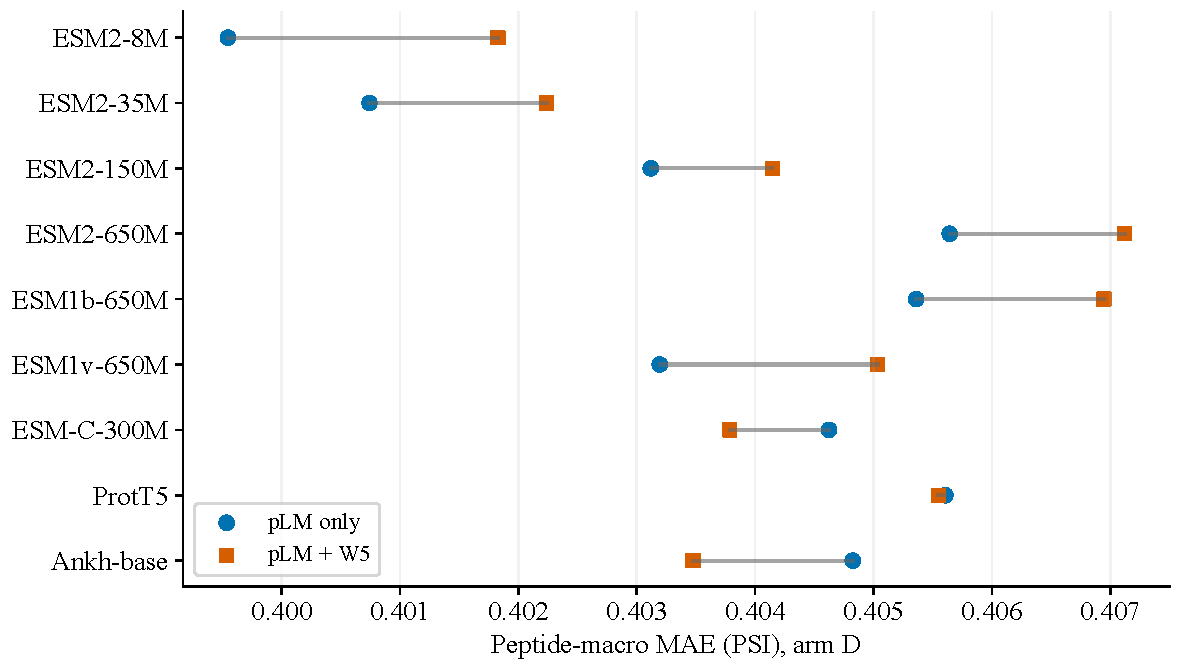
\includegraphics[width=\textwidth]{assets/ch4/fig-campaign-family.pdf}
  \caption[Frozen pLM ridge results under full-range training]{Frozen pLM ridge results under full-range training. Points joined on the same row compare
  explicit context for one checkpoint; the connectors are not confidence intervals.}
  \label{fig:campaign-family}
\end{figure}

Nested selection among the 36 candidates reaches MAE \nCampaignNested{} and positive AUROC
0.8409. Its 15 saved seed/fold choices exactly match the minimum saved inner MSE. ESM2-8M is
selected five times and Ankh three times; several other checkpoints are selected once or twice
(Table~\ref{tab:campaign-nested}). This evaluates a selection procedure, rather than retrospectively
reporting the best outer-OOF family score. Its exploratory MAE difference from the Kaggle W5-D
reference is $-0.01335$, with descriptive group-bootstrap interval $[-0.01719,-0.00967]$.
The cross-runtime comparison does not isolate the causal contribution of pretraining or model size.

\subsubsection{Completed Matched Frozen--LoRA Evaluation}\label{sec:lora-results}
The same-runtime controls now permit a complete adaptation comparison (Table~\ref{tab:campaign-core}).
LoRA-B reaches MAE \nCampaignLoraB{} and positive AUROC \nCampaignLoraAucB{}; LoRA-D reaches
\nCampaignLoraD{} and \nCampaignLoraAucD{}, respectively. Relative to their own frozen controls,
the MAE reductions are \nCampaignGainB\% and \nCampaignGainD\%. All four matched contrasts
retain the favourable direction throughout the adjusted intervals in Table~\ref{tab:campaign-paired}.
Figure~\ref{fig:campaign-core} summarises the matched adaptation results.
This supports adapting this backbone under the specified development protocol; it does not establish
that LoRA will improve every pLM, assay or final deployed model.

\begin{table}[htbp]
  \centering
  \caption[Matched local ESM2-35M results]{Matched local ESM2-35M results. MAE uses all 235 peptides; positive AUROC/AP use
  184 eligible peptides and negative AUROC uses 110. Higher ranking metrics are better.}
  \label{tab:campaign-core}
  % Generated by build_campaign_assets.py; source: research/output-review-2026-11-06/results.json
% SHA256: ad5ba4a4bbffac32e090ca490893b728d9c4239f35484f9b6c6db13c76e94872

{\small\setlength{\tabcolsep}{4pt}
\begin{tabularx}{\textwidth}{Xrrrr}
\toprule
Recipe & MAE & AUROC$+$ & AP$+$ & AUROC$-$ \\
\midrule
Frozen-B & 0.4034 & 0.8263 & 0.4554 & 0.7541 \\
Frozen-D & 0.3904 & 0.8246 & 0.4544 & 0.7667 \\
LoRA-B & 0.3637 & 0.8550 & 0.5517 & 0.7921 \\
LoRA-D & 0.3650 & 0.8536 & 0.5474 & 0.8028 \\
\bottomrule
\end{tabularx}}

\end{table}
\begin{table}[htbp]
  \centering
  \caption[Paired local contrasts: LoRA minus its frozen control]{Paired local contrasts: LoRA minus its frozen control. Confidence intervals use 5,000
  protein-group resamples; 98.75\% intervals adjust a post-hoc family of four comparisons.
  Negative MAE differences and positive AUROC differences favour LoRA.}
  \label{tab:campaign-paired}
  % Generated by build_campaign_assets.py; source: research/output-review-2026-11-06/results.json
% SHA256: ad5ba4a4bbffac32e090ca490893b728d9c4239f35484f9b6c6db13c76e94872

{\small\setlength{\tabcolsep}{4pt}
\begin{tabularx}{\textwidth}{Xrrr}
\toprule
Comparison / metric & $\Delta$ & 95\% CI & 98.75\% CI \\
\midrule
LoRA B $-$ frozen / MAE & -0.0397 & [-0.0470, -0.0324] & [-0.0490, -0.0306] \\
LoRA B $-$ frozen / AUROC$+$ & 0.0288 & [0.0209, 0.0366] & [0.0188, 0.0389] \\
LoRA D $-$ frozen / MAE & -0.0254 & [-0.0318, -0.0191] & [-0.0339, -0.0175] \\
LoRA D $-$ frozen / AUROC$+$ & 0.0289 & [0.0212, 0.0363] & [0.0192, 0.0387] \\
\bottomrule
\end{tabularx}}

\end{table}
\begin{figure}[htbp]
  \centering
  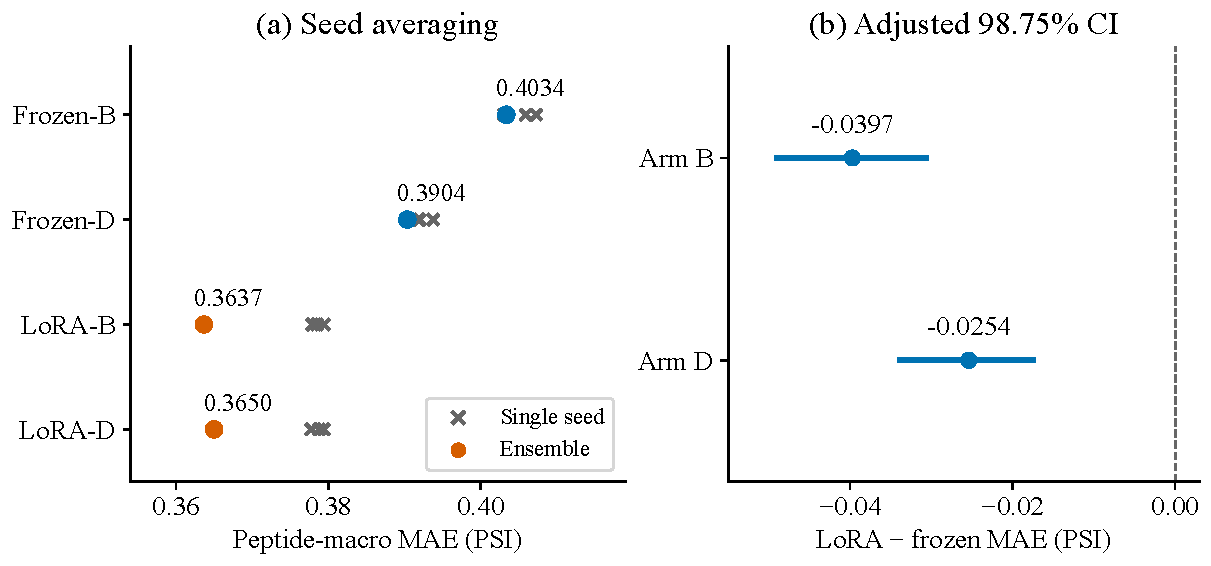
\includegraphics[width=\textwidth]{assets/ch4/fig-campaign-core.pdf}
  \caption[Matched adaptation evidence]{Matched adaptation evidence. (a) Ensemble MAE and individual seed results;
  (b) paired MAE differences with multiplicity-adjusted group-bootstrap intervals.
  The seeds share the outer folds and are not independent cohorts.}
  \label{fig:campaign-core}
\end{figure}

Seed-level MAE differs materially from the ensemble (Table~\ref{tab:campaign-seeds}). For LoRA-B,
single-seed MAEs are about 0.378--0.379, while averaging their predictions gives 0.3637. Consequently,
the ensemble result cannot be assigned to a single checkpoint. All seeds improve on their matched
frozen controls, but shared outer folds prevent treating the seed results as independent replications.
Selected epochs are short: frozen B/D have median 1, LoRA-B median 3 and LoRA-D median 2
(Table~\ref{tab:campaign-epochs}). They are chosen by inner validation, not by outer performance.

Arm choice remains a trade-off. LoRA-D minus LoRA-B MAE is $+0.00133$, with descriptive 95\%
interval $[-0.00295,0.00554]$. The near tie does not establish that restricted training is generally
preferable. Table~\ref{tab:campaign-strata} shows that D improves the PSI $>5$ stratum while B is
better at PSI $\le3$. The highest stratum has no eligible positive-event AUROC peptides, because
its event range is constrained; it still contributes to regression. Stratum intervals are exploratory.

\begin{table}[htbp]
  \centering
  \caption[LoRA peptide-macro MAE by WT-PSI stratum]{LoRA peptide-macro MAE by WT-PSI stratum. The final column is the paired D-minus-B
  difference with a descriptive 95\% protein-group interval; $n$ counts peptides.}
  \label{tab:campaign-strata}
  % Generated by build_campaign_assets.py; source: research/output-review-2026-11-06/results.json
% SHA256: ad5ba4a4bbffac32e090ca490893b728d9c4239f35484f9b6c6db13c76e94872

{\small\setlength{\tabcolsep}{4pt}
\begin{tabularx}{\textwidth}{Xrrrl}
\toprule
WT PSI & $n$ & LoRA-B & LoRA-D & $D-B$ (95\% CI) \\
\midrule
$\le3$ & 91 & 0.3884 & 0.4002 & 0.0118 [0.0043, 0.0194] \\
$(3,4]$ & 85 & 0.3812 & 0.3815 & 0.0003 [-0.0056, 0.0064] \\
$(4,5]$ & 36 & 0.3092 & 0.3033 & -0.0059 [-0.0138, 0.0027] \\
$>5$ & 23 & 0.2863 & 0.2613 & -0.0250 [-0.0439, -0.0056] \\
\bottomrule
\end{tabularx}}

\end{table}

LoRA-B also has lower MAE than the Kaggle frozen-ESM CNN-D by 0.02069 PSI, with descriptive
interval $[-0.02659,-0.01489]$. This is useful for prioritising candidates, but head architecture,
runtime and adaptation all differ. The matched local contrasts provide the more specific evidence
for adapter training. Kaggle and local ESM2-35M ridge controls are numerically close but are kept
separate, rather than relabelled as additional independent seeds.

% Numbers: assets/ch4/build_progress_assets.py from the independent saved-OOF audit.
\subsubsection{Residual Diagnostics and Difficult Cases}\label{sec:residual-diagnostics}
A new calculation directly from the saved OOF predictions examines where the matched adaptation
helps and fails. These are post-hoc descriptive diagnostics on W, not new independent tests or
subgroup significance claims. Figure~\ref{fig:progress-residuals} retains every peptide, including
\nProgressBPepWorse{} that worsen with LoRA-B and \nProgressDPepWorse{} with LoRA-D.
The corresponding counts with lower MAE are \nProgressBPepBetter{} and \nProgressDPepBetter{}.
After averaging peptide differences within a protein group, B improves \nProgressBGrpBetter{}
groups and worsens \nProgressBGrpWorse{}; D improves \nProgressDGrpBetter{} and worsens
\nProgressDGrpWorse{}. Group counts describe a different weighting from peptide-macro MAE.

\begin{figure}[htbp]
  \centering
  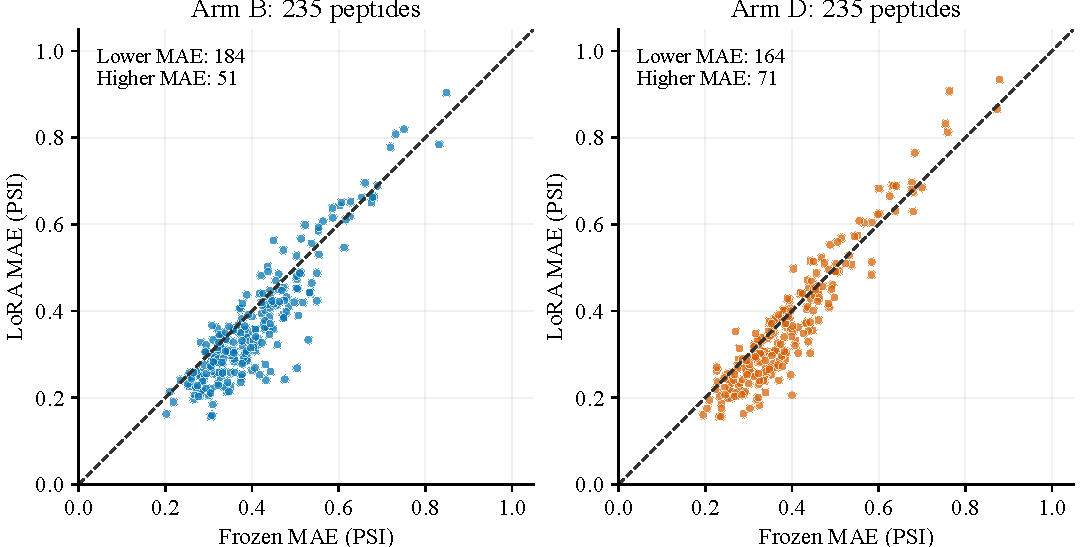
\includegraphics[width=\textwidth]{assets/ch4/fig-progress-residuals.pdf}
  \caption{Matched per-peptide OOF errors for the three-seed ensembles on W. Each point is one
  peptide; points below the dashed equality line favour LoRA. Both panels use common scales.
  The spread is observed heterogeneity, not a confidence interval.}
  \label{fig:progress-residuals}
\end{figure}

Removing each protein group in turn leaves the peptide-macro LoRA-minus-frozen MAE difference
negative: ranges are \nProgressBLeaveGroup{} for B and \nProgressDLeaveGroup{} for D.
This rules out a reversal driven by removal of any one recorded group; it does not establish
robustness to simultaneous removal of several related groups or to unobserved biological dependence.
LoRA-B fold MAEs range from 0.3384 to 0.3862 and LoRA-D from 0.3431 to 0.3882, so a global
average should not be interpreted as uniform performance. The worst LoRA-B peptide, CCDC17 tile~9,
has MAE 0.9035 versus 0.8486 for frozen-B. It remains a failure case despite the average gain.

\begin{table}[htbp]
  \centering
  \caption{OOF MAE conditional on the measured effect class ($\Delta=\Delta$PSI).
  Each metric averages errors within each eligible peptide, then over peptides in that class.
  Support counts differ from ranking eligibility, which requires at least three cells of each class.}
  \label{tab:progress-effect-errors}
  % Generated by build_progress_assets.py; descriptive OOF diagnostics.
% Source: research/progress-review-2026-11-06/local-audit.json
% SHA256: 2ea1d4235a4123bdcd0411f788f1356be6fe99b835105d1743700cf2670195a5
{\small\setlength{\tabcolsep}{3.5pt}
\begin{tabularx}{\textwidth}{Xrrrrrrr}
\toprule
Effect & Cells & Pep./grp. & Fr.-B & LoRA-B & Fr.-D & LoRA-D & Zero \\
\midrule
$-1<\Delta<1$ & 108,782 & 235/221 & 0.3270 & 0.2879 & 0.3045 & 0.2843 & 0.3031 \\
$\Delta\ge1$ & 12,053 & 198/190 & 0.8187 & 0.7997 & 0.8972 & 0.8479 & 1.4155 \\
$\Delta\le-1$ & 1,577 & 151/144 & 1.2407 & 1.0385 & 1.1394 & 0.9510 & 1.2320 \\
\bottomrule
\end{tabularx}}

\end{table}

Table~\ref{tab:progress-effect-errors} shows substantially greater errors for large effects than
for neutral cells. For $|\Delta\mathrm{PSI}|\ge1$, LoRA-B and D have MAE 0.8970 and 0.9084,
respectively, versus 1.4127 for zero, over 13,630 cells, 232 peptides and 218 groups. The positive
class has 12,053 cells; the negative class has only 1,577. LoRA-B's cell-micro signed residual
($\widehat{\Delta}-\Delta$) is $-0.9504$ for positive cells and $+1.0449$ for negative cells.
The direction is consistent with underestimating effect magnitude, but does not isolate a biological
mechanism or distinguish model shrinkage from measurement noise. These signed residuals have
different weighting from the peptide-macro absolute errors in the table.

\begin{table}[htbp]
  \centering
  \caption{Three largest absolute cell errors for LoRA-B on W, selected after inspection.
  Positions are within the measured peptide; measured and predicted values are $\Delta$PSI.
  These illustrate failures and are not clinical or mechanistic case validations.}
  \label{tab:progress-largest-errors}
  % Generated by build_progress_assets.py; descriptive OOF diagnostics.
% Source: research/progress-review-2026-11-06/local-audit.json
% SHA256: 2ea1d4235a4123bdcd0411f788f1356be6fe99b835105d1743700cf2670195a5
{\small\setlength{\tabcolsep}{4pt}
\begin{tabularx}{\textwidth}{Xrrrrr}
\toprule
Peptide & Fold & Position & Change & Measured & Predicted \\
\midrule
P32881\_IFNA8\_5 & 2 & 17 & Y$\to$F & 3.2866 & -0.1573 \\
P13942\_COL11A2\_20 & 1 & 18 & R$\to$I & 3.1698 & -0.2479 \\
P32881\_IFNA8\_5 & 2 & 17 & Y$\to$M & 3.0830 & -0.2058 \\
\bottomrule
\end{tabularx}}

\end{table}

The difficult cases in Table~\ref{tab:progress-largest-errors} include sign reversals for strongly
stabilising measured substitutions. Post-hoc tables by mutant amino acid and by WT--replacement
pair are retained in the accompanying audit with support counts. Their uneven support and shared
protein contexts prevent interpreting a high subgroup error as a causal residue-specific mechanism.


\subsubsection{Probability Calibration and Locked Transfer}\label{sec:campaign-calibration-transfer}
Table~\ref{tab:campaign-calibration} distinguishes probabilistic quality from ranking. Both LoRA
arms lower multiclass Brier score relative to their frozen controls and the inner-prior baseline.
The peptide-macro LoRA-minus-frozen Brier differences are $-0.01572$ for B and $-0.01349$ for D,
with descriptive 95\% group intervals $[-0.01986,-0.01152]$ and $[-0.01736,-0.00970]$.
However, positive-event ECE increases. Reliability curves in Figure~\ref{fig:campaign-calibration}
show overconfidence in high-probability bins, which contain fewer cells. A lower Brier score does
not establish uniformly better calibration. The model cards currently mark these as CV-only
calibrators and leave the final serving-model identifier list empty; model-specific lineage and
final refitting remain necessary before inference integration.

\begin{table}[htbp]
  \centering
  \caption[Out-of-fold three-class probability evaluation]{Out-of-fold three-class probability evaluation. Brier is the unnormalised sum across
  three classes; lower values are better. The prior uses inner-validation class frequencies.
  ECE refers only to the positive event and uses ten equal-width bins.}
  \label{tab:campaign-calibration}
  % Generated by build_campaign_assets.py; source: research/output-review-2026-11-06/results.json
% SHA256: ad5ba4a4bbffac32e090ca490893b728d9c4239f35484f9b6c6db13c76e94872

{\small\setlength{\tabcolsep}{4pt}
\begin{tabularx}{\textwidth}{Xrrrr}
\toprule
Recipe & Brier micro & Brier macro & Prior micro & ECE$+$ \\
\midrule
Frozen-B & 0.1789 & 0.1787 & 0.2006 & 0.0129 \\
Frozen-D & 0.1795 & 0.1794 & 0.2006 & 0.0114 \\
LoRA-B & 0.1631 & 0.1630 & 0.2006 & 0.0163 \\
LoRA-D & 0.1659 & 0.1659 & 0.2006 & 0.0165 \\
\bottomrule
\end{tabularx}}

\end{table}

The locked transfer set contains 39,234 R/A/S substitutions across 1,410 peptides and 730 protein
groups, with no recorded group overlap with W or scanning development data. Only the fixed W5-D
recipe is evaluated. It obtains MAE \nCampaignTMaE{}, compared with \nCampaignTZero{} for
predicting zero. The paired difference is \nCampaignTDelta{} with 95\% interval
\nCampaignTCI{}, so the average regression advantage is not resolved. Positive AUROC is
\nCampaignTAuc{} on 338 eligible peptides and AP is 0.6011; negative AUROC is only 0.5176 on
85 eligible peptides. Regression, positive ranking and negative ranking therefore have different
transfer behaviour.

\begin{table}[htbp]
  \centering
  \caption[Locked W5-D transfer by WT PSI]{Locked W5-D transfer by WT PSI. $n$ counts peptides and $n_{+}$ counts peptides
  eligible for positive-event AUROC. The zero predictor provides a regression reference.}
  \label{tab:campaign-transfer}
  % Generated by build_campaign_assets.py; source: research/output-review-2026-11-06/results.json
% SHA256: ad5ba4a4bbffac32e090ca490893b728d9c4239f35484f9b6c6db13c76e94872

{\small\setlength{\tabcolsep}{4pt}
\begin{tabularx}{\textwidth}{Xrrrr}
\toprule
WT PSI & $n$ & W5-D MAE & Zero MAE & $n_{+}$ \\
\midrule
$\le3$ & 524 & 0.3819 & 0.4319 & 231 \\
$(3,4]$ & 323 & 0.3918 & 0.4158 & 89 \\
$(4,5]$ & 306 & 0.3998 & 0.3843 & 18 \\
$>5$ & 257 & 0.4428 & 0.3470 & 0 \\
\bottomrule
\end{tabularx}}

\end{table}
\begin{figure}[htbp]
  \centering
  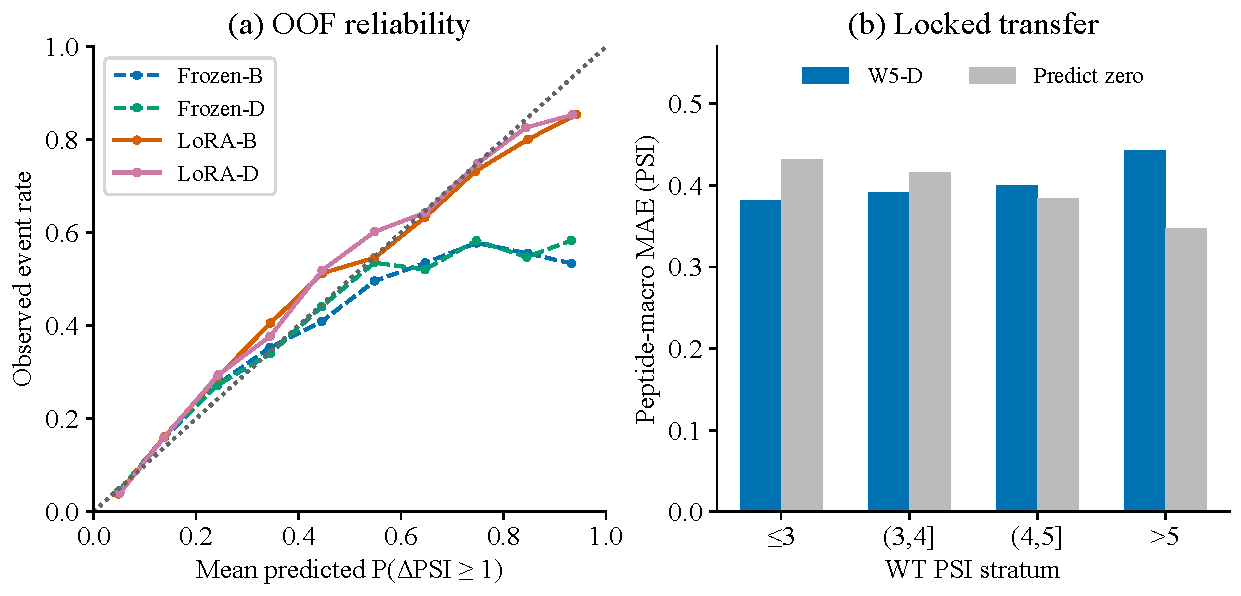
\includegraphics[width=\textwidth]{assets/ch4/fig-campaign-calibration-transfer.pdf}
  \caption[Probability and transfer limitations]{Probability and transfer limitations. (a) Development OOF positive-event reliability,
  with the diagonal indicating agreement; (b) locked W5-D transfer MAE by WT PSI.
  T uses a different population and does not evaluate LoRA.}
  \label{fig:campaign-calibration}
\end{figure}

The transfer failure is concentrated in high-WT-PSI peptides: above 5, W5-D MAE is 0.4428 versus
0.3470 for zero (Table~\ref{tab:campaign-transfer}). Across T, the observed positive-cell rate is
0.0512, below mean predicted probability 0.0895. Although the three-class Brier score of 0.1291
beats the development-prior baseline of 0.1348, positive probabilities shift upward relative to
the observed rate. T contains only R, A and S replacements (25,479, 9,278 and 4,477 cells), uses
replicate-1 labels and comes from a previously explored same-laboratory source. These results
do not demonstrate independent external validity, clinical utility or transfer of the LoRA gain.

\subsubsection{Additional Controls and Practical Consequences}
The complete Kaggle record also contains composition, unordered-context, substitution-only,
learning-curve, quality-weighting and scanning-label controls (Table~\ref{tab:campaign-all}).
The substitution-only ridge encodes WT and replacement identity as separate one-hot blocks;
despite its saved ``pair'' name, it does not add interaction terms or W5 positions. In arm D it
reaches MAE 0.4017 and AUROC 0.8092, compared with ordered W5 at 0.4078 and 0.8319.
Composition gives 0.4075/0.8109 and unordered context 0.4060/0.8258. Thus explicit ordering
improves positive ranking in these controls without minimising MAE. W3-B similarly has slightly
lower MAE than W5-B (0.4331 versus 0.4336), while W5-B has higher positive AUROC
(0.8312 versus 0.8280). Context benefit depends on the outcome being optimised.

Training-coverage controls A/B/C/D give W5 MAEs 0.4711, 0.4336, 0.4177 and 0.4078 as the
training threshold increases from 3 to 4 to 5 to the full range. These are full-range evaluations,
so their values cannot be compared directly with the old restricted benchmark. Scanning augmentation
of ridge gives MAE 0.4047 using replicate 1 and 0.4048 using the replicate mean, versus 0.4078
without the extra source. The matched scanning CNNs likewise reach about 0.3872/0.3873.
The observed point differences do not establish an advantage from averaging replicate labels.

For W5-D, mean single-seed MAE decreases from 0.4413 at one-quarter training data to 0.4189 at
one-half, 0.4107 at three-quarters and 0.4078 at full size. Ensemble MAEs are 0.4154, 0.4113,
0.4083 and 0.4078. The large ensemble gain at small fractions must not be misread as a learning
curve of one fitted model. Fractional training subsets vary by seed, so their ensemble can have
seen a union larger than the stated fraction. The frozen ESM CNN-D improves MAE for 156 of
235 peptides, grouped
into 150 of 221 protein groups, relative to W5-D; the advantage is not universal.

The scanning pre-training comparison also examines the 20 substitution-pair types present
in scanning and the other 360 types. Improvements are observed outside the 20 scanned pair types,
but the subsets remain part of the same development population. This is evidence about the tested
representation and label-transfer procedure, not a newly independent transfer cohort. These controls
and the negative weighting result remain in the full appendix rather than being removed from the
record after a stronger model appears.

Recorded completed-attempt durations total about 14.1 hours for frozen tuning and 36.0 hours for
LoRA tuning, versus about 1.4 hours for the 540 ridge fits (Table~\ref{tab:campaign-timing}).
Paused/resumed jobs may omit earlier attempt time, so these totals are not exact GPU-active time
or the wall-clock duration of the campaign. They still identify adaptation as the main recorded
computational cost. The transfer inference timer is for prediction only and does not include fitting,
feature preparation, downloads or service startup.

The executable research graph is finished. The next research tasks are reviewed external/structure
inputs, independent transfer checks and a compatible final serving refit, calibrator, lineage card and
export. The application tasks remain separate. A report marked complete is neither release acceptance
nor automatic promotion of the lowest development MAE.
